\documentclass{article}
\usepackage[left=2cm, right=2cm, top=2cm]{geometry}
%%%%%%%%%%%%%%%%%%%%%%%%%%%%%%%%%% PACKAGES %%%%%%%%%%%%%%%%%%%%%%%%%%%%%%%%%%
\usepackage{minted}                     % Code
\usepackage{graphicx}                   % PNGs
\usepackage{algorithm}
\usepackage{algpseudocode}              % Algorithms
\usepackage{hyperref}                   % Hyperlinks
\hypersetup{
    colorlinks,
    linkcolor=black
}

%%%%%%%%%%%%%%%%%%%%%%%%%%%%%%%%%%%%%%%%%%%%%%%%%%%%%%%%%%%%%%%%%%%%%%%%%%%%%%%

\pagenumbering{gobble}

\title{\textbf{Homework #1}}
\author{MacMillan, Kyle}
\date{September 28, 2018}


\begin{document}

\maketitle
\addcontentsline{toc}{section}{Title}

\newpage
\pagenumbering{roman}   % Set TOC page numbering to lowercase roman numerals
\tableofcontents
\addcontentsline{toc}{section}{Table of Contents}


\newpage
\listoffigures
\addcontentsline{toc}{section}{\listfigurename}
\listofalgorithms
\addcontentsline{toc}{section}{\listfigurename}


\newpage
\pagenumbering{arabic}  % Set content page numbering to arabic numerals
% Setup Hyperlinks for the rest of the document
\hypersetup{
    colorlinks,
    citecolor=blue,
    filecolor=black,
    linkcolor=blue,
    urlcolor=blue
}

\section{Problem 1}}
\setcounter{page}{1} % Set the page counter to 3
\textit{What are the identity values for the operators}: $\&\&,\ ||,\ |,\ ^\wedge $?

\begin{itemize}
    \begin{tabular}{@{}ll}
    \item $\&\&$ &: 1\\
    \item $||$ &: 0\\
    \item $|$ &: 0\\
    \item $^\wedge$ &: 0\\
    \end{tabular}
\end{itemize}



\section{Problem 2}
\textit{Suppose OpenMP did not have the reduction clause. Show how to implement an efficient parallel reduction by adding a private variable and using the critical pragma.}
\inputminted{c++}{problem2.cpp}

\begin{figure}[h]
    \centering
    \begin{minipage}{0.7\textwidth}
        \centering
        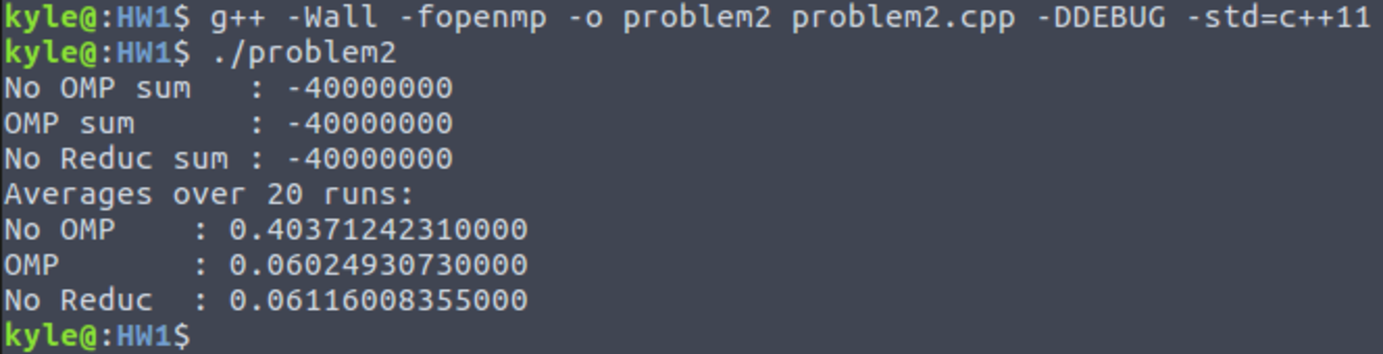
\includegraphics[width=0.95\textwidth]{Problem2debug}
        \caption{Example debug output.}
        \label{fig:p2debug}
    \end{minipage}\hfill
    \begin{minipage}{0.3\textwidth}
        \centering
        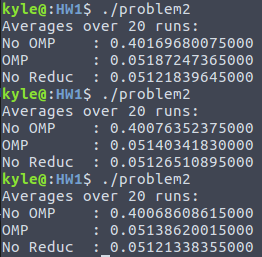
\includegraphics[width=0.95\textwidth]{Problem2_60}
        \caption{Better performance without reduction.}
        \label{fig:p2}
    \end{minipage}
\end{figure}

As can be seen in the figures the sums are performing as expected. An interesting, and expected outcome is that in Figure~\ref{fig:p2debug} it takes 0.06 seconds to run $OMP$ and $No\ Reduc$ but in Figure~\ref{fig:p2} it takes 0.05 seconds. The $No\ OMP$ takes 0.40 seconds regardless. The reason for this behavior is that $OMP$ uses the cores you give it and at the time of recording the first figure the browser was open and running a video. When I recorded the second Figure I had closed my browser to maximize performance for multi-core processing. The $No\ OMP$ section of code was only running on one core, so it did not care that I had a video playing.


\section{Problem 3}
\subsection{Problem 3a}
\begin{minted}{c++}
    #pragma omp for
    for(i = 0; i < (long) sqrt(x); ++i) {
        a[i] = 2.3 * i;
        if (i < 10) 
            b[i] = a[i];
    }
\end{minted}

\subsection{Problem 3b}
This code section is not suitable for OpenMP because of the \&\& operator in comparison.
Per the \hyperlink{https://www.openmp.org/wp-content/uploads/openmp-4.5.pdf}{OpenMP documentation} \S2.6, p53:\\\\
\begin{tabular}{@{}ll}
$test$-$expr$ & One of the following:\\
& $var\ relational$-$op\ b$\\
& $b\ relational$-$op\ var$\\\\

$relational$-$op$ & One of the following:\\
& $<$  \\
& $<=$ \\
& $>$  \\
& $>=$ \\
\end{tabular}

\subsection{Problem 3c}
This code can be ran with OMP but it is dependent on whether or not $foo()$ is threadsafe.
\begin{minted}{c++}
    #pragma omp for
    for(i = 0; i < n; ++i) {
        a[i] = foo(i);
    }
\end{minted}

\subsection{Problem 3d}
asdf

\subsection{Problem 3e}
asdf

\subsection{Problem 3f}
asdf

\subsection{Problem 3g}
asdf

\subsection{Problem 3h}
asdf



\section{Problem 4}
asdf


\newpage
\section{Problem 5}
\textit{If the address of the nodes in a hypercube has n bits. How many nodes can it be at the most and how many edges does each node have? 
Give an algorithm that routes a message from node u to node v in this k-node hypercube in no more than log(k) steps.}\\

Hypercubes are generalized by dimensionality. A hypercube address containing n-bits will exist in n dimensions ($d$). The maximum number of nodes is determined by $d$, and is defined as $\[2^d\]$. A trait of hypercubes is that each node will have $d$ edges. The total amount of edges would be defined as $d * \[2^{d-1}\]$. The number of nodes you have to travel between $u$ and $v$ is equal to the number of differing bits.\\ 
For example:
\begin{itemize}
    \begin{tabular}{@{}llll}
    \item 000 & $=>$ & 111 & : 3\\
    \item 001 & $=>$ & 100 & : 2\\
    \item 110 & $=>$ & 011 & : 2
    \end{tabular}
\end{itemize} 

\noindent Therefore a traversal algorithm would be:\\
\begin{algorithm}[H]
\caption{Move from node $u$ to $v$}
\label{alg:Prob5}
\Statex Initialize Variables
\State $i\gets 0$
\State $current\_bit\gets u[i]$
\State $left\_bit\gets u[i]$
\While {$i < dimension(hypercube)$}
    \State $current\_bit\gets u[i]$
    \If {current\_bit $=$ v[$i$]}
        \State $i\gets i+1$
    \Else
        \State $route(current\_bit)$ \Comment{Routes to neighbor node containing the correct bit}
    \EndIf
\EndWhile
\end{algorithm}

If built properly there will only be one node the algorithm can route to during the $route(current\_bit)$ section. Essentially we look at the left-most bit and if it is the same we move to the next bit, if it is different we must move to a new node. There will only be one node available because if they are on the same dimension they would have the same bit in that slot. For example on a 3-dimensional hypercube 000 to 100 looks at the left bit and sees it is on a different dimension. There is only one node connected to 000 that follows the format 1xx, so that is the only place it can go. If we wanted to route from 000 to 010 we would identify we are on the correct 3rd dimension, then look at the middle bit. From there we would see a need to move in the second dimension. There is only one connected node that matches in the second dimension, so that is where it would go.


\newpage
\section{Graduate Assignment}
\textit{Do a search on Shuffle-exchange network topology.  
Draw the network with 16 processor nodes (carefully numbering each node binary and showing what is a shuffle link, what is an exchange link).  If k is the number of digits in the binary address, how many nodes (n) are there?  With n nodes what is the diameter (d) of the networks, the bisection width (b) and how many edges/node?}\\

When you first drew a shuffle-exchange network (also sometimes called butterfly network) I immediately thought that looked like a sorter I came up with in 300. I later learned that sort wasn't something I had uniquely developed and was in fact a \href{https://en.wikipedia.org/wiki/Bitonic_sorter}{bitonic sort}. 


\end{document}
